\chapter{Algorytmy}

\section{Centralność w grafach}

W teorii grafów wskaźniki centralności informują o najbardziej znaczących wierzchołkach grafu. Ich przykładowymi zastosowaniami mogą być: znalezienie lidera, przywódcy spośród danej grupy osób, ustalenie kluczowego elementu infrastruktury sieciowej lub miejskiej bądź znalezienie osobnika o największym potencjale do roznoszenia choroby. Istnieje wiele odmiennych wskaźników centralności. Zrealizowany projekt implementuje trzy z nich: Closeness Centrality, Betweenness Centrality oraz Pagerank ( jedna z odmian Eigenvector Centrality)



\section{Betweenness Centrality}

Określa kluczowość wierzchołka w zakresie komunikacji - przechodność, pośredniczenie. Czyli w jakim stopniu dany wierzchołek jest spoiwem dla danej sieci. Jest to miara o bardzo wielkiej wartości, gdyż dzięki niej można znaleźć punkty krytycznej sieci bądź grafu.

\subsection{Algorytm wyznaczania}
\begin{enumerate}
\item Wyznaczyć ilość najkrótszych ścieżek między wierzchołkami $u$ i $v$ ( $d_{uv}$ )
\item Wyznaczyć ilość najkrótszych ścieżek między wierzchołkami $u$ i $v$, które przechodzą przez wierzchołek $w$ ( $d_{uv}(w)$ )
\item Suma stosunków  oznacza stopień centralności wierzchołka $w$ $$c_b(w) = \sum_{u \neq v \neq w} \frac{d_{uv}(w)}{d_{uv}}$$
\end{enumerate}

\FloatBarrier
\subsubsection{Przykład}
\begin{figure}[h]
\centering
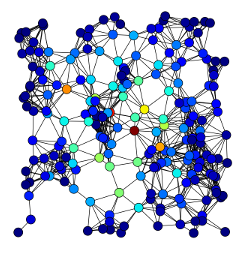
\includegraphics[scale=1.0]{betweenness_demo}
\caption{Działanie Betweenness Centrality  na przykładowym grafie}
\end{figure}
\FloatBarrier


\section{Closeness Centrality}

Jest to stopień bliskości. Określa jak blisko (daleko) wierzchołek ma do pozostałych w grafie. Wysoki stopień biskości świadczy o dobrej własności propagacji informacji w grafie - element ten szybko rozprowadzi daną wiadomość (wirusa itp) po całej sieci.


\subsubsection{Algorytm wyznaczania}
\begin{enumerate}
\item Wyznaczyć odległości pomiędzy wierzchołkiem $u$ a pozostałymi wierzchołkami w grafie $v$  ( $d_{uv}$ )
\item W zależności od rodzaju grafu zsumować otrzymane odległości:
\begin{enumerate}
\item Dla grafów rzadkich $$ c_c(u) = \frac{1}{\sum d_{uv} }$$
\item Dla grafów silnie połączonych $$ c_c(u) = \sum_{u \neq v} \frac{1}{d_{uv} }$$
\end{enumerate}
\end{enumerate}

\FloatBarrier
\subsubsection{Przykład}
\begin{figure}[h]
\centering
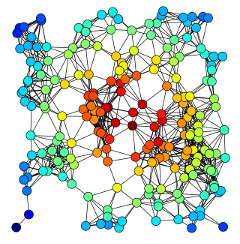
\includegraphics[scale=1.0]{closeness_demo}
\caption{Działanie Closeness Centrality  na przykładowym grafie}
\end{figure}
\FloatBarrier

\section{Eigenvector Centrality - Pagerank}
Określa wpływ, oddziaływanie wierzchołka na pozostałe w grafie. Wykorzystuje nie tylko ilość połączeń danego wierzchołka z innymi, a przede wszystkim ich jakość. Wartości przypisane do każdego z wierzchołków bazują na koncepcji w której wysoko ocenione wierzchołki bardziej wpływają na ostateczną ocenę połączonego wierzchołka, niż te, których ocena jest niska. Jedną z odmian Eigenvector Centrality jest algorytm PageRank. Poniżej przedstawiono uproszczony algorytm jego działania.

\subsubsection{Algorytm wyznaczania}
\begin{enumerate}
\item Wyznaczyć ilość wierzchołków w grafie ($N$)
\item Wyznaczyć stopień każdego z wierzchołków ($l(u)$)
\item Zainicjować wartości początkowe dla każdego wierzchołka wartością początkową ($c_e(u) = 1$)
\item Określić współczynnik tłumienia, zwykle wynosi on około 0.85 ( $d = 0.85$ )
\item Obliczyć nową wartość PageRank każdego wierzchołka $$ c_e(u) = \frac{1 - d}{N} + d\sum_{v \in B_u} \frac{c_e(v)}{l(v)}$$ $B_u$ oznacza zbiór wszystkich wierzchołków, które odnoszą się do wierzchołka $u$
\end{enumerate}

\FloatBarrier
\subsubsection{Przykład}
\begin{figure}[h]
\centering
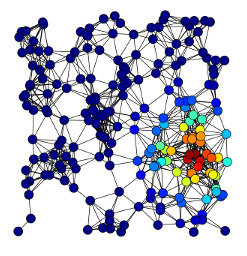
\includegraphics[scale=1.0]{pagerank_demo}
\caption{Działanie Eigenvector Centrality  na przykładowym grafie}
\end{figure}
\FloatBarrier